
%\newpage
\section{Měření frekvence}
\label{sec:frequency}

Počínaje verzí 1.10k lze měřit frekvenci a toto vybrat pomocí ovládacího menu.
Normální měření frekvence se provádí počítáním padajících hran vstupního signálu T0 (PD4).
Je to provedeno s počítadlem 0 (COUNTER 0) po dobu jedné vteřiny.
K udržení přesné vteřiny se používá čítač 1 s před-děličem frekvence CPU 256:1.
16-bitový čítač ATmega může s před-děličem v jednom průchodu i při \(16MHz\) CPU frekvencí vypočítat jednu vteřinu.
Pro spuštění a zastavení čítače 0 jsou použity srovnávací B a A registry čítače 1.
K předejití dodatečné nejistotě času v dotazech, jsou zde  používané, pro obě srovnávací události,
rutiny služby přerušení. Časové zpoždění u těchto rutin služby přerušení je přibližně stejné.
K udržení přesné sekundy je konstantní časová prodleva irelevantní.
Analýzou kódu assembleru lze časovou nerovnost vyrovnat.
Při frekvencích pod \(33kHz\) se k měření přidává měření doby periody.
Toto měření se provádí po normálním měření frekvence.
přitom bude čas určitého počtu změn úrovně vstupu PCINT20 (PD4) měřen čítačem 0.
Pro měření periody by měla být, jak záporná, tak i kladná šířka impulsu
nejméně \(10\mu s\)  v každém období dlouhá.
Čítač 0 běží s plnou taktovou CPU rychlostí, což poskytuje pro jednu periodu \(125ns\).
Větším počtem změřených období lze rozlišení přesnosti ještě zlepšit.
Při 125 periodách (250 změnách úrovně) je výsledkem středního rozlišení pro periodu již \(1ns\).
Aby nevznikla žádná nepřesnost při startu a zastavení čítače 0, je čítač 0 spuštěn při první změně úrovně
PCINT20 a po zadaném čísle, přes stejnou rutinu služby přerušení, zase zastaven.
Počet období je zvolen tak, aby doba měření činila přibližně 10 milionů taktů.
Chybová složka taktu je pak \(0,1~ppm\). U \(8MHz\) je doba měření přibližně 1,25 vteřin.
Z takto určeného středního období se vypočte frekvence s vyšším rozlišením.
Pro kontrolu byly naměřeny dva testery proti sobě.
Pouze s testerem 2 byly generovány zkušební frekvence a byly měřeny frekvencemi testeru 1.
Poté bylo měření opakováno s obrácenými testery.
Na obrázku \ref{fig:freq-ppm} jsou zobrazeny výsledky.
Takřka konstantní relativní odchylky lze vysvětlit malými frekvenčními rozdíly obou křemenů.

\begin{figure}[H]
\centering
\includegraphics[width=.8\textwidth]{../GNU/frequency-ppmCZ}
\caption{Relativní chyba při měření frekvence}
\label{fig:freq-ppm}
\end{figure}

\subsection{Kalibrace frekvence pomocí GPS nebo přijímače GLONASS}
Jemná změna frekvence testeru je možná pomocí proměnného kondenzátoru (trimmer \(5-25pF\)) u krystalu.
Pro referenci jsem úspěšně testoval vteřinový signál (1PPS) s GPS {\textbf UP501} přijímačem od společnosti {\textbf Fastrax Ltd.} a
pomocí přijímače GPS/GLONASS {\textbf GNS701} od {\textbf Global Navigation Systems GmbH} úspěšně testoval.
Naměřená doba může být nastavena pomocí trimru přesně na \(1000,000ms\).
Pouze poslední zobrazená číslice se může o 1 lišit.
Samozřejmě, závisí frekvence k na teplotě.
To je důvod, proč nemůžete očekávat velmi dobrou dlouhodobou stabilitu.
Obrázek \ref{fig:GPS-1PPS} ukazuje obvody používané s UM232 USB-sériovým převodníkem pro
připojení modulů přijímače k ​​počítači.
Převodník UM232 napájí obvod s provozním napětím \(5V\) ale také s \(3,3V\) z USB napájení.
\\Při provozu přijímače není nutné připojení k počítači.
Musí být pouze zaručena dodávka \(5V\) s USB zásuvky.

\begin{figure}[H]
  \begin{subfigure}[b]{.5\textwidth}
    \centering
    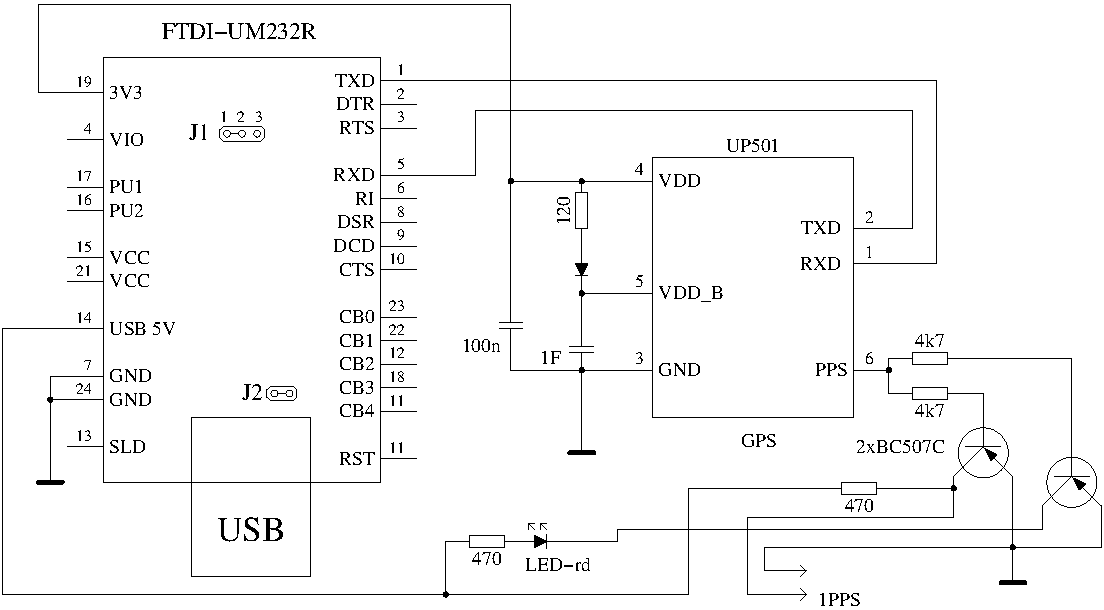
\includegraphics[width=.95\textwidth]{../FIG/GPS_UP501.pdf}
    \caption{GPS}
  \end{subfigure}
  ~
  \begin{subfigure}[b]{.5\textwidth}
    \centering
    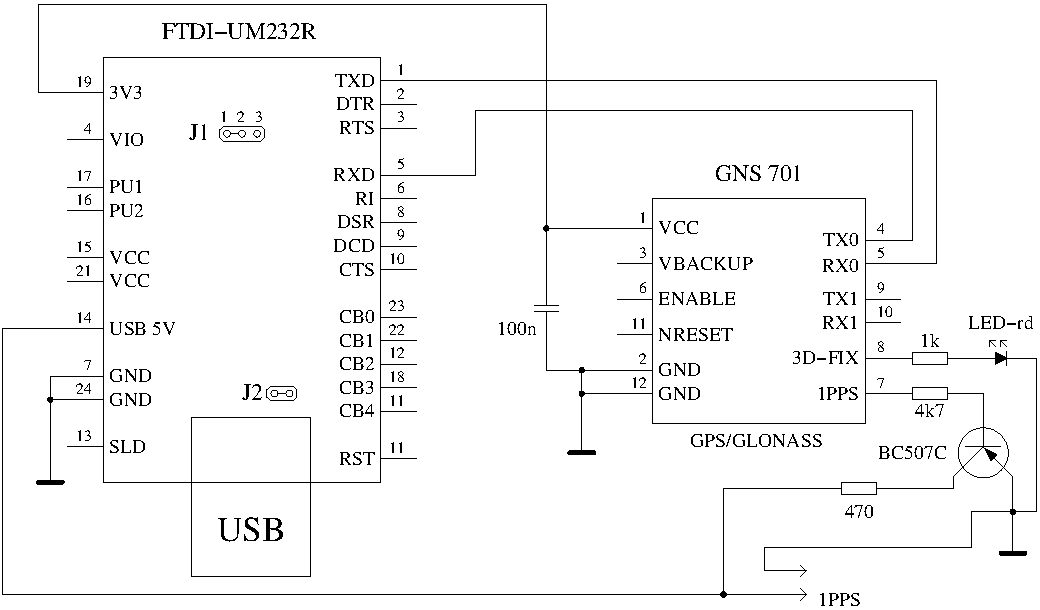
\includegraphics[width=.95\textwidth]{../FIG/GPS_GNS701.pdf}
    \caption{GPS/GLONASS}
  \end{subfigure}
  \caption{Vteřinová pulzní generace s GPS přijímači}
  \label{fig:GPS-1PPS}
\end{figure}

\subsection{Kalibrace frekvence krystalu s hodinovým modulem}

K naladění krystalové frekvence testeru, je výměna jednoho ze dvou krystalových kondenzátorů
proti trimru s požadovanou nastavitelnou kapacitou nutná.
Výhodou použití hodinových modulů oproti GPS nebo GLONASS frekvenčních tuningových modulů je to,
že nemusíte mít žádný jasný výhled na oblohu a GPS družice.
Nastavení lze provádět téměř kdekoli.
Zkoušel jsem moduly hodinky s DS3231 a nápisem ,,ZS-042''.
Uvedené moduly jsou nejpravděpodobnější z čínské výroby a nepoužívají DS3231SN čip,
ale DS3231M čip s MEMS rezonátorem (MEMS = Mico Electro Mechanical System).
Mimochodem, DCP1301 čip také používá podobný MEMS rezonátor.
Obrázek~\ref{fig:DS3231M} zobrazuje jeden z použitých modulů.

\begin{figure}[H]
\centering
\includegraphics[width=.6\textwidth]{../PNG/DS3231M.jpg}
\caption{Jeden z uvedených DS3231 modulů}
\label{fig:DS3231M}
\end{figure}

Čip DS3231SN však používá jako časovou základnu hodinový křemen s \(32768Hz\).
Pro obě varianty čipů DS3231 je měřeno teplotní chování frekvence kmitání pomocí měření vnitřních teplot čipu,
aby byla dosažena dobrá frekvenční přesnost v širokém teplotním rozmezí.
Bohužel je ale \(32kHz\) vyvedený signál na modulu u varianty DS3231M čipu pro kalibraci nevhodný.
U čtyř přítomných modulů byly naměřeny kmitočty \(32641Hz\), \(32710Hz\), \(32730Hz\) a \(32748Hz\).
Všechny frekvence byly od skutečně očekávaných přesných \(32768Hz\) daleko vzdáleny.
Připojením těchto modulů k Arduino UNO systému, můžete také připojit signál 1PPS (\(1Hz\)) výstup na SQW výstup.
Tento výstup je však v periodě tak stabilní, že ho lze použít pro kalibraci.
Datový list zaručuje pro DS3231M přesnost \(\pm 5ppm\) v celém rozsahu teplot pro
výstup 1PPS \(-45\celsius\)  do \(+85\celsius\), zatímco přesnost \(32kHz\) výstupu je
zaručena pouze na \(\pm 2,5\%\) (\(25000ppm\)).
V datovém listu DS3231SN je v rozmezí teplot od \(-40\celsius\) do \(+85\celsius\) slíbená
přesnost \(\pm 3.5ppm\) a pro rozsah teplot od \(0\celsius\) do \(+40\celsius\) přesnost \(\pm 2ppm\).
Čip DS3231SN používá jako časovou základnu hodinový krystal s frekvencí \(32768Hz\),
který s přepínatelnými kapacitami, drží stabilní kmitočet v širokém teplotním rozmezí.
Se známou teplotní charakteristikou krystalu a na čipovém integrovaném teplotním čidlu je frekvence převážně konstantně udržována.
Pro zkoumání tohoto čipu jsem všechny DS3231M čipy vyměnil za DS3231SN.
Pro čerstvě kalibrovaný tester s \(16MHz\) krystalem, je měření frekvence pro všechny
čtyři moduly stejnou frekvenci \(32.76800kHz\) se zřídka uvedenou odchylkou od \(0.03Hz\).
To odpovídá odchylce cca \(1ppm\).
Mimochodem, 1 Hz zlomky jsou zobrazeny pouze tehdy, když je frekvence vypočtena z měření periody.
Aby bylo možné měřit \(32768Hz\) touto metodou, změnil jsem hranici pro měření doby od \(25kHz\) na \(33kHz\).
Tato přesnost zobrazení frekvence může být samozřejmě dosažena pouze tehdy, pokud je zdroj kmitočtu stabilní a s nízkým šumem.
Při použití signálu odvozeného z RC generátoru výrazně kolísají výsledky měření.
